\chapter{Design part}

\section{Description of the design architecture}

\subsection{Agents}

We can define 3 types of agents :\\

\begin{itemize}
	\item[{\bf Attendant,}] somebody who is here to attend concert
	\item[{\bf Vigil,}] someone who keep an eye on people. We can have regular
	vigils, and specialized vigils like medics, who help injured people
	\item[{\bf Shopkeepers,}] sell goods to attendants people
\end{itemize}

\begin{figure}[h]
	\begin{center}
		
\includegraphics[width=0.7\textwidth]{img/agents.png}
	\end{center}
	\caption{Agents representation}
\end{figure}

\subsection{Environment}

The environment will be represented in 2D. The map is a simple area, filled with
fixed entities and different kind of people. A single entrance/exit is present,
with emergency exits all around the area.\\

Entities can be listed as follows:\\

\begin{itemize}
	\item[{\bf Stages,}] where the bands play, and people gather around it
	\item[{\bf Obstacles,}] trees, barriers, etc...
	\item[{\bf Toilets,}] distinction between men’s and women’s
	\item[{\bf Food stands,}] where people go eat and drink
	\item[{\bf Shopping stands,}] where people can shop souvenirs
	\item[{\bf One entrance/exit + emergency exit,}] Where you can enter or
	leave the festival
\end{itemize}

\begin{figure}[h]
	\begin{center}
		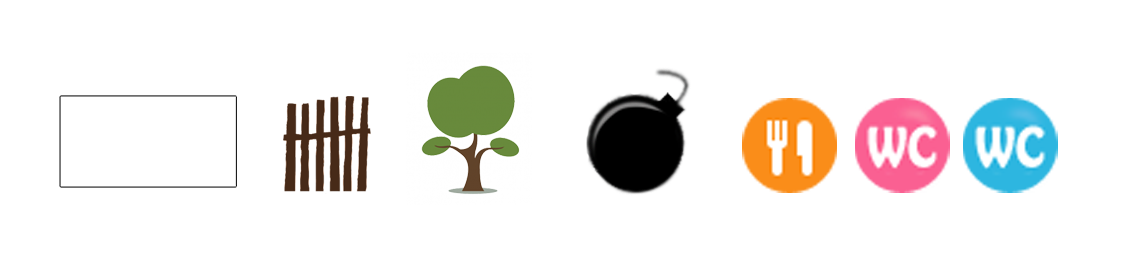
\includegraphics[width=0.7\textwidth]{img/environment.png}
	\end{center}
	\caption{Entities representation}
\end{figure}

\subsection{GUI}

The GUI part is in both sub-packages, framework and motion. It is called from
the launch of the MainProgram class. It contains all the references to graphical
data (sprites), and it manages the capture of the mouse to set the bomb
somewhere on the map. Apart from that, it just draws the scene at each step of
the program, when all agents have performed their actions.

\subsection{Behaviours}

For each agent, we can specified differents behaviour :\\

\begin{itemize}
	\item[{\bf Attendants}] each person has a list of concert he wants to see,
	he will try to go to each of them. Different schedules can be made :\\
	
		\begin{itemize}
			\item Regular schedule, one concert each hour, no conflict, the
			schedule will only be interrupted by natural needs (food, toilets,
			drink)
			\item Groupie schedule, one group in particular, skip the previous
			concert to be in the first row, then regular schedule
			\item Conflicted schedule : some concerts are in conflict, so the
			person will see x\% of the first one and 100-x\% of the second one
		\end{itemize}


 	Outside of schedules, people can act differently :\\
		
		\begin{itemize}
			\item Regular people, drink a bit, eat a bit, use the restrooms, go
			to concerts from the beginning to the end
			\item Drugged people, slow motion, can slow the evacuation process
			\item Angry people, various reasons (alcohol, pogos, fights), can
			hurt others people. People hurted should be evacuated by vigils as
			soon as seen
			\item A few, randomly selected can be heavy drinkers and start to
			act totally randomly (should be stopped by vigils as soon as seen by
			one)
			\item Idiot people, take the evacuation as an opportunity to be on
			the front row
		\end{itemize}

	\item[{\bf Vigils}] As presented above, there is two types of vigils :
		\begin{itemize}
			\item Regular vigils : stay at the same place all the day, have
			a sight of seeing to detect drunk people and angry people, maybe
			rotation of given people at given posts
			\begin{itemize}
				\item[\emph{Passive}] stationed near his post ( stage
				supervisory, entry body check)
				\item[\emph{Active}] motion until in range of troublemakers
				then warning or neutralization, back to original post after
				operation success
			\end{itemize}
			\item Medics : same as vigils but for injured people
		\end{itemize}

	\item[{\bf Shopkeepers}] sells goods to people, stay behind the stand the
	all night and evacuate when needed
\end{itemize}

Apart from those specific behaviors for each type of agent, there is also
a panic behavior, which is triggered by the user (events defined
below).

\begin{itemize}
	\item Augmentation of maximal speed
	\item Reduction of perception field
	\item Following crowd direction until perception of emergency exit
\end{itemize}


\subsection{Tools}

The application will be written in Java, in a Maven project. For the interface,
it will be in 2D (aerian view), using Swing. To manage the multi-agent aspect of
the project, Janus 1.0 will be used. The teamwork was optimized with the help of 
the SCM Git.\\

Sources can be found here :
\href{https://github.com/zarov/EurockSimulation}{https://github.com/zarov/EurockSimulation}

\section{Class diagram}

Given the important size of the simulation, and to be coherent between everything, we designed a class diagram as follow :

\newpage

\begin{figure}[h]
	\begin{center}
		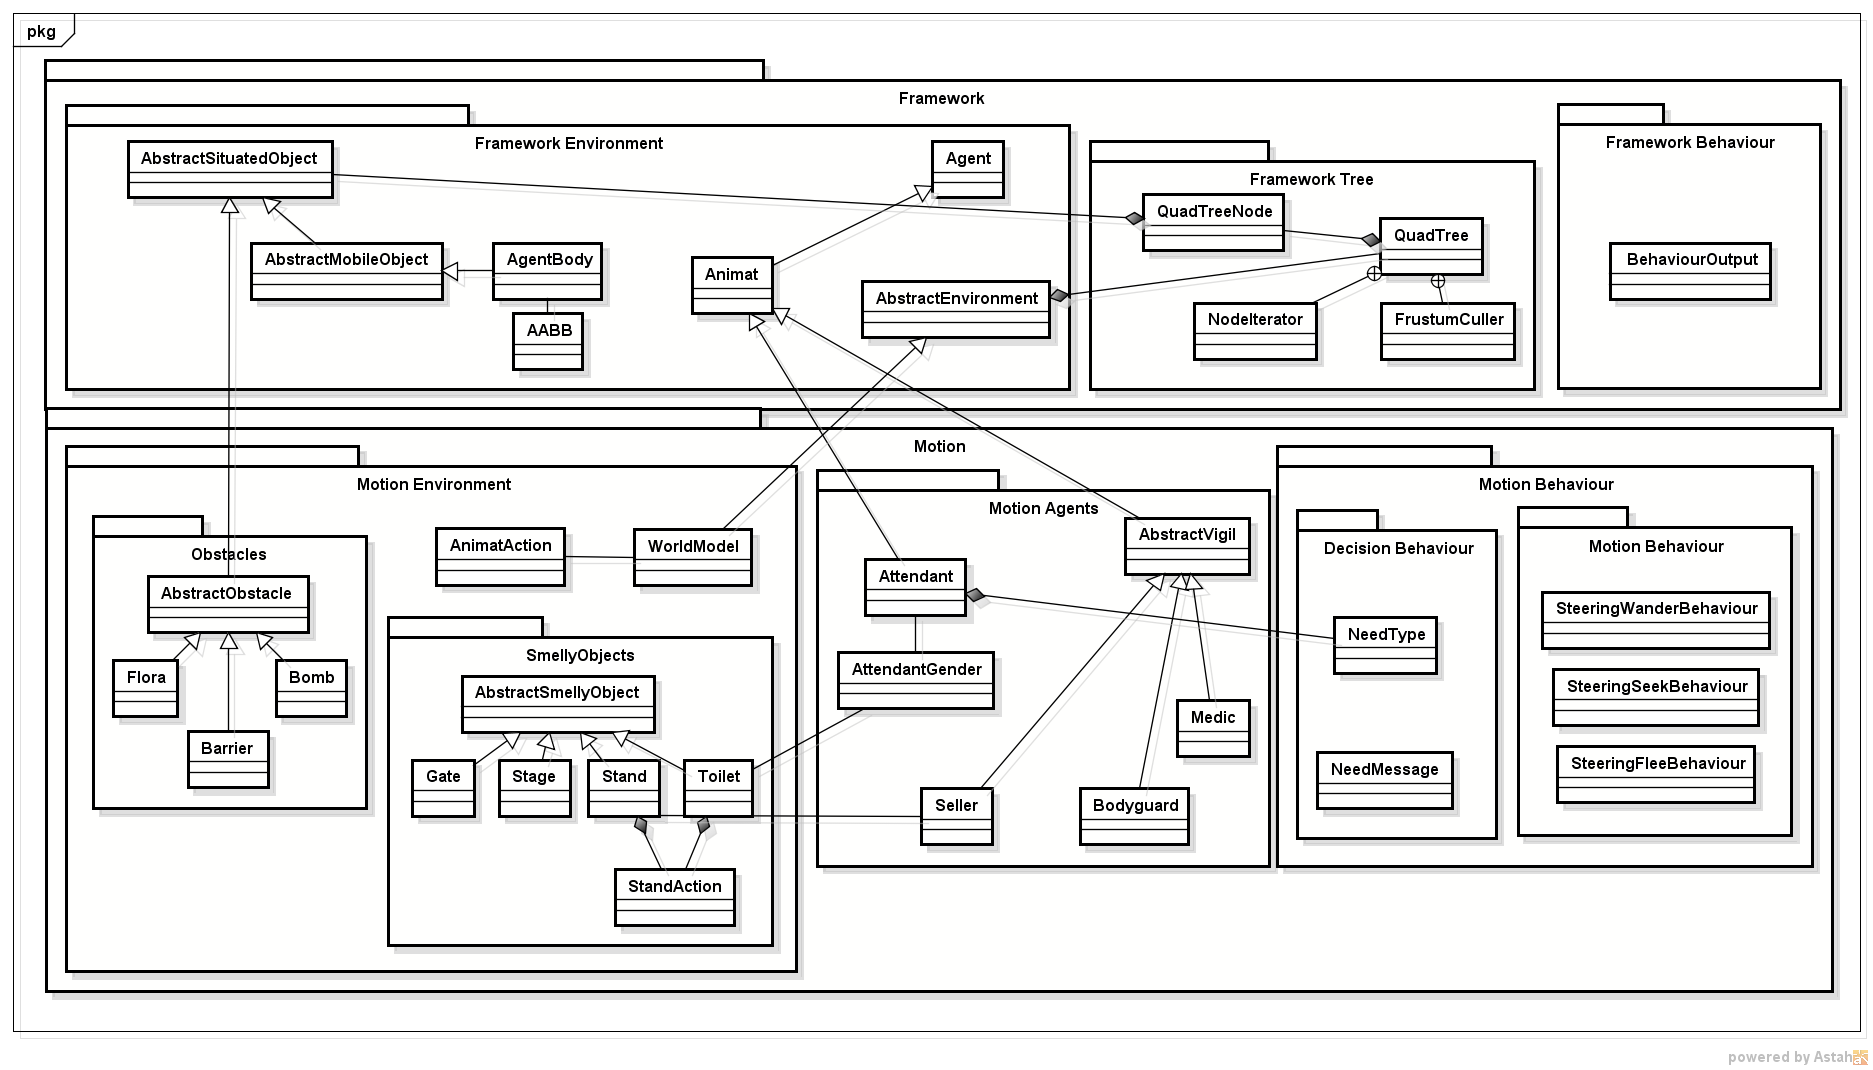
\includegraphics[width=0.72\textheight, angle=90]{img/classdiagram.png}
	\end{center}
	\caption{Class diagram}
\end{figure}

\newpage

\section{Design choice and explanations}

\subsection{Decision making}

Attendants are the only agents that follow a real decision making process.
Attendant movements are guided by their instant need. Implemented needs are thirst, hunger, seeing gig need and going to bathroom need. Each attendant moves in direction of the object that will satisfy its higher need; once satisfied, another need takes over that lead to a new movement target.

\begin{figure}[h]
	\begin{center}
		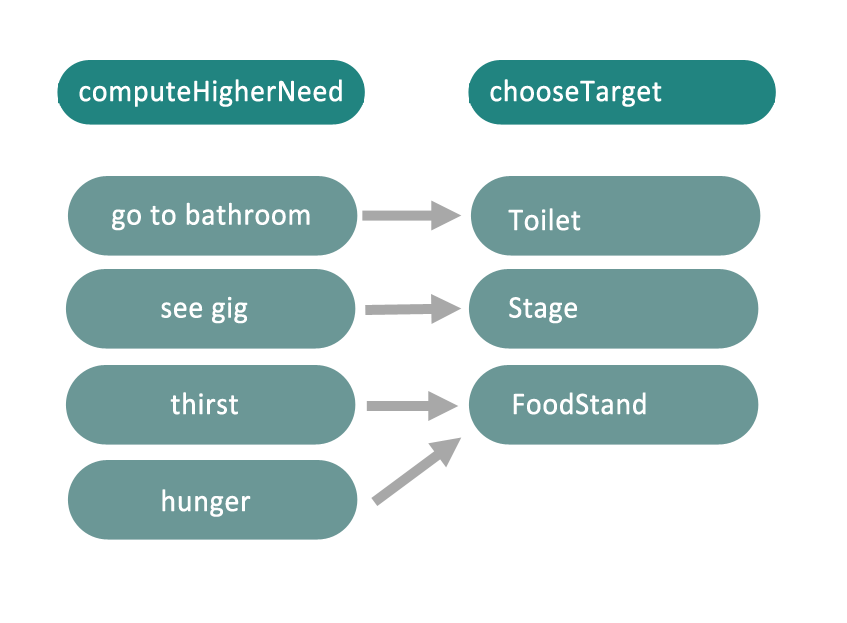
\includegraphics[width=0.8\textwidth]{img/decisionmaking.png}
	\end{center}
	\caption{Decision making graph}
\end{figure}

\newpage

\subsection{Classical and panic behaviors}

\paragraph{Attendant Behaviour}

\begin{itemize}
	\item Update his need function of messages received
	\item Optional: increase his need randomly
	\item Get perception function of its frustum
	\item Choose a seek target function of its higher need and perceptions
	\item Choose a flee target (closer obstacle) for collision avoidance
	\item Run both flee and seek behavior function of the target
\end{itemize}

\begin{figure}[h]
	\begin{center}
		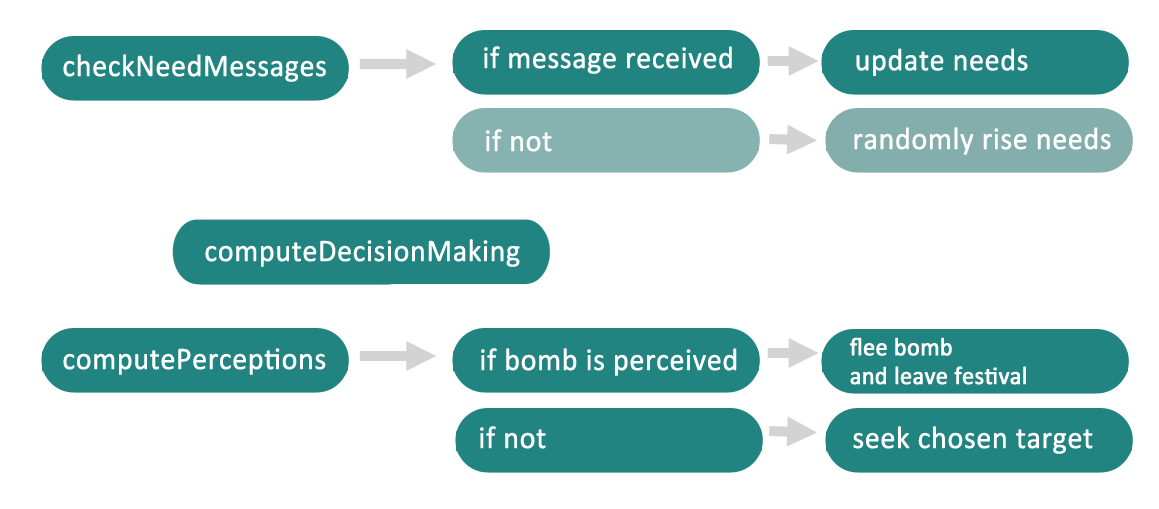
\includegraphics[width=0.8\textwidth]{img/attendantbehaviour.png}
	\end{center}
	\caption{Attendant behavior graph}
\end{figure}

\paragraph{Seller Behaviour}

\begin{itemize}
	\item Get perception
	\item Check if bomb is seen
	\item Else send a message to the attendant on to of the stand stack
\end{itemize}

\begin{figure}[h]
	\begin{center}
		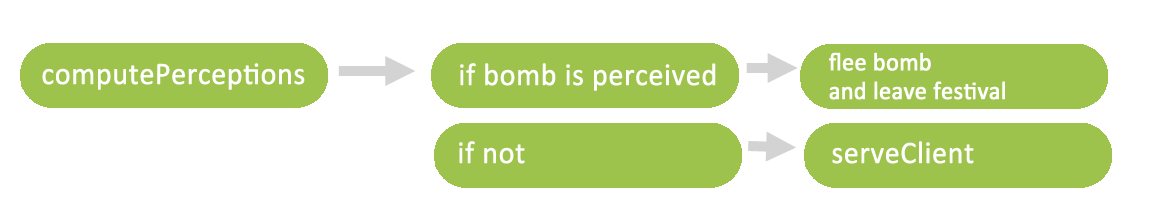
\includegraphics[width=0.8\textwidth]{img/sellerbehaviour.png}
	\end{center}
	\caption{Seller behavior graph}
\end{figure}

\paragraph{Medic Behaviour}

\begin{itemize}
	\item Get perception
	\item Check if an attendant is hurt
	\item In case one is, rush to him until he his healed or transported to safety
\end{itemize}

\paragraph{Bodyguard Behaviour}

\begin{itemize}
	\item Get Perception
	\item Stay near stage
	\item Check if an attendant has a drunk behaviour
	\item Guide him out of the gig far from the stage
	\item Tag team with medic to protect hurted attendant from the crowd
\end{itemize}

\newpage

\section{Used techniques}

\subsection{Quadtree structure}

To store environment’s objects, we could use a Grid, but this structure is too
basic and can not contain all the data of the environment. If the simulation
needs to fit reality, there will be at least 80.000 attendants, and a lot of
other people as vigils, medics etc… So a lot of data needs to be handle, and a
simple Grid can’t do that. A Grid is also for discrete movements, and there
isn’t a need for such movements.\\

A Tree is more adapted, especially a QuadTree, that can divide the space in 4 in
each of his node. Compared to a Grid, it is way faster, because the search can
be focused on one corner of a chosen node at each level. On a theoretical level,
a Grid has a complexity of $O(n)$ while a Tree as one of $O(\log n)$. It is the
final choice made to manage the environment.\\

The implementation of the QuadTree is an adaptation of the QuadTree seen in
courses. The structure is, of course, the same as every QuadTree : each node has
a set of children (maximum four), and each child has a unique parent. The root
of the tree is the entire map of the Eurockéennes. There is various methods
within the tree. First, a classic Iterator has been implemented, which traverses
the node in a depth-first iteration. There is also a find function which takes
as an argument an object of the world, based on the box of elements and nodes.
As AABB boxes are used, it is possible to tell if a box is inside a node. The
algorithm is as follows :\\

\begin{algorithm}[H]
	\While{iterator has next}{
		node <= iterator next
		\eIf{not(node.box contains object)}{
			\tcc{as the node doesn’t contain the object, we can remove children
			of the node}
			iterator remove 4 next
			}{
			\If{node is leaf}{
				break
			}
		}
	}
\end{algorithm}

\subsection{Frustum culler}

In the tree, there is also a function that allow to get the objects in the
perception field of an agent. And if we want to be more efficient, it can remove
objects that the agent doesn’t see. So basically it works the same as the find
function, but instead of looking if a node contains an object, it’s searching if
the object is in the frustum, a AABB box to represent the perception field,
after being sure that the frustum at least intersects with the node in which
it’s taking a look at. So at the end the algorithm is as this :\\

\begin{algorithm}[H]
	\While{iterator has next}{
		node <= iterator next
		\If{frustum intersects node.box AND contains node.object}{
			add object to percepts
		}
	}
\end{algorithm}

\subsection{Agents communication}

In order to communicate between agents, we used the mailbox system offered by
Janus library. This system allowed us to realize interactions between people in
one particular case : attendant’s food delivery. Indeed once a hungry festival
attendant reached a stand to get some food, he places himself in the stand
queue. Stand seller then peek the first client in the queue and send him several
messages containing actions that will apply on his needs, for example -7 on
drinking need and +3 on going to bathroom need.

\subsection{Collision avoidance}

One of the main aspect of the UV is the collision management between agents,
themselves and environment. But as we were focused on managing the needs and
behaviours of each agent, we didn’t take time to implement correctly a good
collision avoidance. Hence there is only collision avoidance with stages and the
gate.\\

The algorithm is simple : a stage has an influence zone which repulse agents
that are in a determined radius. If an agent has a stage in his perception
field, a flee target is set, to avoid the collision with the object. After the
behaviours are computed, the flee target is added to the computed movement. The
final movement of the agent is then adapted to the collision.

\subsection{Bomb implantation}

The bomb is considered as an obstacle, Agents will then flee away from it as soon as they see it. A timer is set in the GUI, which will be displayed on the screen. The WorldModel will take care of decreasing this timer, and once it arrives at 0, the WorldModel will hurt the Agents in range to be hurt and kill the ones closer to the bomb. Both ranges are defined as a propriety of the bomb class.

\section{Encountered problems}

\subsection{AgentBody/AgentAddress}

Find an body knowing its animat address, in laboratory work examples, was quite
easy to realize thanks to a Map structure linking both classes. Since in our
case, only SituatedObjects are stocked in the QuadTree structure, finding the
body corresponding to an address without going through the entire QuadTree and
test every of the bodies became a problem.

\subsection{The toilet issue}

Solution used to act on attendant needs from a foodstand was to delegate the task of applying need changes to the seller belonging to this stand. Indeed as an agent it was able to send a message to the attendant. In the case of toiletstand though, no agent was there to send the message to the agent allowing him to go elsewhere.\\

The only way we have think of to solve this issue was to create a unique invisible Agent to which is assigned a set of all toilets of the map and whose unique live behaviour is to check the queue of every toilet stand and send a message to each attendants on top of those queues.

\subsection{Smelly Object}

Our first intuition about how to guide agents to the object in adequation to their need was to use the concept of smelly objects. The principle is that interesting objects emits a smell decreasing function of the distance. People interested in finding one object will detect the object proper smell and go in direction of the strongest smell.\\

At last this technique involved too much complications, and according to attendant perceptions ranges and the numerous stands, agents are able to find their way to the appropriate stand thanks to their perceptions only.

\section{Benchmark}

\subsection{QuadTree}

So as to be certain of the structure reliability we run JUnit tests on the structure and its different iterators. That method was very helpful in a way that we could check at any new code inclusion if something has been damaged, especially if we consider that iterators use AgentBody’s attributes which can potentially be modified during the project development.\\

In these tests, the QuadTree supports really well the insertion of thousands of entities (environment and agent) with no problem. It was tested with 100.000 of trees (as flora) without impact on performance (a few seconds). It is ok to have such results, because it is the initialization of the simulation, so it doesn’t impact afterward.\\

The find function and the frustum culler have more weight on performance. Even if the data structure is a QuadTree, which gives a high gain in computation time, if an object to search for is far in the Tree, it can take a lot of time to get to it. It is the main impact on the simulation, because when the number of agents increases, the number of computation inside the Tree increases too. It isn’t a problem from the data structure itself, but more from the algorithm of search. If some criterias and parameters are added inside the object of the Tree, it may improve the computation. In all cases, it is a problem of optimization.

\subsection{Agents}

In real life, there is approximately between 80.000 and 100.000 attendants a day at the festival. We can count also between 1.000 and 2.000 workers during the three days. So in theory, the simulation need to work with these numbers. Let’s try with different number of people.\\
 
For these tests, workers are alone on their own stand. If we increase the numbers of workers, while staying at a ratio 1 worker for 50 attendants (same as reality), it doesn’t influence very much (a few ms), because a worker has few computation to do.\\

Results of benchmark :\\

\begin{itemize}
	\item[200 attendants] $\rightarrow$ step computed between 52 and 80 ms
	\item[500 attendants] $\rightarrow$ step computed between 171 and 246 ms
	\item[1000 attendants] $\rightarrow$ step computed around 600 ms
	\item[5000 attendants] $\rightarrow$ step computed around 11 and 13 s
\end{itemize}